%%%%%%%%%%%%%%%%%%%%%%%%%%%%%%%%%%%%%%%%%%%%%%%%%%%%%%%%%%%%%%%%%%%%%%%%%%%%%%%%
%2345678901234567890123456789012345678901234567890123456789012345678901234567890
%        1         2         3         4         5         6         7         8

\documentclass[letterpaper, 10 pt, conference]{ieeeconf}  % Comment this line out if you need a4paper

%\documentclass[a4paper, 10pt, conference]{ieeeconf}      % Use this line for a4 paper

\IEEEoverridecommandlockouts                              % This command is only needed if 
                                                          % you want to use the \thanks command

\overrideIEEEmargins                                      % Needed to meet printer requirements.



% See the \addtolength command later in the file to balance the column lengths
% on the last page of the document

% The following packages can be found on http:\\www.ctan.org
%\usepackage{graphics} % for pdf, bitmapped graphics files
%\usepackage{epsfig} % for postscript graphics files
%\usepackage{mathptmx} % assumes new font selection scheme installed
%\usepackage{times} % assumes new font selection scheme installed
\usepackage{amsmath} % assumes amsmath package installed
\usepackage{amssymb}  % assumes amsmath package installed
\usepackage{accents}
\usepackage{graphicx}
\usepackage[font=small,labelfont=bf]{caption}
\usepackage{subcaption}
\usepackage{float}
%\usepackage{framed}
\usepackage{cite}
\usepackage{algorithm}
\usepackage{algorithmic}

% Some table tweaks to increase spacing
%\setlength{\tabcolsep}{8pt}		% Default is 6pt
\renewcommand{\arraystretch}{1.2}	% Default is 1.0


%%%%%%%%%%%%%%%%%%%%%%%%%%%%%%%%%%%%%%%%%%%%%%%%%%%%%%%%%
\title{\LARGE \bf
	Explosive Motion with Compliant Actuation Arrangements in Articulated Robots
}



%%%%%%%%%%%%%%%%%%%%%%%%%%%%%%%%%%%%%%%%%%%%%%%%%%%%%%%%%
\author{Roel Djajadiningrat$^{1}$, Wesley Roozing$^{2}$ and Nikolaos G. Tsagarakis$^{2}$% <-this % stops a space
	\thanks{$^{1}$ Roel Djajadiningrat is a M.Sc student at the Department of Mechanical Engineering, TU Delft and a visiting student at Istituto Italiano di Tecnologia;
		{\tt\ r.djajadiningrat@student.tudelft.nl}
	}%
	\thanks{$^{2}$Wesley Roozing and Nikolaos G. Tsagarakis are with the Department of Advanced Robotics,
		(Fondazione) Istituto Italiano di Tecnologia, via Morego,
		30, 16163 Genova, Italy.
		{\tt\ \{wesley.roozing, nikos.tsagarakis\}@iit.it}
	}%
}


%%%%%%%%%%%%%%%%%%%%%%%%%%%%%%%%%%%%%%%%%%%%%%%%%%%%%%%%%
\begin{document}

\maketitle
\thispagestyle{empty}
\pagestyle{empty}


%%%%%%%%%%%%%%%%%%%%%%%%%%%%%%%%%%%%%%%%%%%%%%%%%%%%%%%%%
\begin{abstract}

This paper presents the optimisation of explosive jumping motions on a 3-DoF leg prototype. The leg is based on the recently introduced asymmetric compliant actuator scheme, in which a series-elastic main drive is augmented with a secondary parallel adjustable compliant branch with significantly different stiffness and energy storage capacity properties. The leg prototype implements two such actuation configurations, one of which includes a biarticulated branch, and they are compared to conventional series-elastic based actuation. An optimisation problem is formulated to optimise the joint trajectories and elastic element pretension to maximise jumping height. A simulation study demonstrates that the biarticulated configuration yields maximum jumping height, and achieves the highest peak joint power. Compared to series-elastic based actuation, the augmented leg jumps 4\% higher with a monoarticulated parallel compliance configuration while using less energy, and over 10\% higher in biarticulated configuration.

\end{abstract}


%%%%%%%%%%%%%%%%%%%%%%%%%%%%%%%%%%%%%%%%%%%%%%%%%%%%%%%%%
\section{INTRODUCTION}
In the past robots were found predominantly in static industrial settings, but in recent years they have been introduced to more dynamic settings, operating with and among humans. This change is accompanied by a change in requirements. One of the primary challenges is enabling robots to match human performance in terms of motion. This requires light-weight actuation that allows for energy efficient explosive motion, large peak force, and matching motion planning and control. A prime example of an explosive motion in humans is the vertical jump.

Several approaches have been investigated over the years to design robotic systems capable of energy efficient explosive motion. Traditional rigid actuation poses problems with weight and resulting insufficient performance. Therefore, systems with compliant properties have been proposed. The compliant `Bow Leg' hopping robot \cite{zeglin1999bow} used a curved leaf spring made of laminated fibreglass, and showed that low power motors can be sufficient active actuation when parallel energy storage is used. A small bipedal jumping robot `Mowgli' \cite{niiyama2007mowgli} used compliant tendons antagonistic to pneumatic artificial muscles, enabling it to jump as high as 0.5\,m. A switchable form of Parallel-Elastic Actuation (\textit{PEA}) was shown to combine the benefits of compliant properties while maintaining a high degree of control and energy efficiency when the parallel compliance is not needed \cite{liu2015spear}. Besides actuation parameters, the importance of optimised joint trajectories was shown to be a major factor in improved energy efficiency \cite{velasco2013soft, babivc2009biarticulated}. Furthermore, biarticulated actuation, in which a single muscle spans multiple joints simultaneously, has been shown to drastically increase explosive performance in humans \cite{schenau1989rotation,prilutsky1994tendon}. In robotics, comparative jumping experiments with single-actuator biarticulated robots and multiple-actuator robots also demonstrate increased performance of biarticulated configurations \cite{oshima2007jumping,babivc2009biarticulated,hyon2002development}.

% some old sentences we don't have space for
% It was shown that accurate and stable force control can be achieved with Series Elastic Actuation (\textit{SEA}) \cite{pratt1995series}.
% Analytical research on Series-Elastic Actuation (SEA) shows that a \textit{SEA} performing a hammering task can reach a speed up to four times that of the actuator’s prime mover \cite{garabini2011optimality}.
%A comparison with \textit{PEA} showed that a hopper with \textit{SEA} is more energetically efficient than one with \textit{PEA} when looking at positive actuator work and electrical work \cite{yesilevskiy2015comparison}.

Recently, Roozing et al. \cite{roozing2016development, roozing2016design, roozing_design_2018} presented the development and control of a novel Asymmetric Compliant Actuation (\textit{ACA}) scheme characterised by large energy storage capacity, enabling efficient mobility, as well as a novel method to select design parameters of such structures to maximise energy efficiency of multi-DoF articulated robots using these concepts. This paper extends these works, contributing by using the \textit{ACA} concept to execute optimised jumping motions on the model of the recently developed 3-DoF leg prototype \cite{roozing_design_2018}. Two augmented actuation designs, one of which includes a biarticulated tendon spanning ankle and knee, are compared to state-of-the-art Series Elastic Actuation (\textit{SEA}). The augmented leg jumps 4\% higher in monoarticulated configuration while using less energy, and over 10\% higher in biarticulated configuration. Furthermore, the biarticulated case shows higher peak joint power and joint-to-joint power transfer. These results demonstrate significant benefits of such actuation approaches in explosive motions.

This paper is structured as follows. Sec. \ref{sec:legDesign} describes the 3-DoF leg prototype, the actuation concepts, and the three different actuation configurations. Sec. \ref{sec:modelling} describes the forward and inverse dynamics of the leg. Sec. \ref{sec:dynamicOptimisation} introduces the optimisation problem, followed by the results and their discussion in Sec. \ref{sec:results}. Finally, concluding remarks are given in Sec. \ref{sec:conclusions}.


%%%%%%%%%%%%%%%%%%%%%%%%%%%%%%%%%%%%%%%%%%%%%%%%%%%%%%%%%
\section{Leg Design}
\label{sec:legDesign}

\subsection{Asymmetric Compliant Actuation}
\label{subsec:ACA}
The Asymmetric Compliant Actuation (\textit{ACA}) concept consists of a combination of two parallel actuation branches with very different power and stiffness properties, as shown in Fig. \ref{fig:ACA}. The Power Branch (\textit{PB}) is a rotary \textit{SEA} which consists of a high power motor \textit{M1} in series with a torsional elastic element denoted as \textit{SE}. The Energy Storage Branch (\textit{ESB}) consists of a lower power motor \textit{M2}, with a high reduction linear transmission which transfers its power to the joint through a unidirectional series elastic element denoted as \textit{PE}. Compared to the series-elastic element in the \textit{PB}, the \textit{ESB} elastic element can store a significantly larger amount of energy. In biarticulated configurations (bottom of Fig. \ref{fig:ACA}), the \textit{PB} drives the joint directly, while the \textit{ESB} tendon spans a second joint by means of a free pulley, as depicted in Fig. \ref{fig:ACA}. As such, the tendon elongation depends on the configuration of both joints, and the tendon exerts torque on both joints.

% Figure asymmetric compliant actuation branches
\begin{figure}[ht]
	\centering
	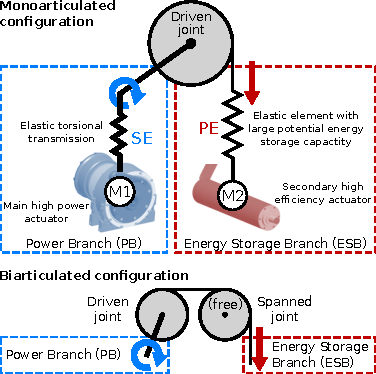
\includegraphics[width=0.75\linewidth]{actuationConcept}
	\caption{The Asymmetric Compliant Actuation (\textit{ACA}) concept, shown in monoarticulated (top) and biarticulated (bottom) configurations.}
	\label{fig:ACA}
\end{figure}

\subsection{3-DoF Leg Prototype}
The design of the 3-DoF leg prototype is inspired by the human lower limb. The dimensions and mass distribution of the human limb were investigated, and compared with those of existing humanoid designs such as WALK-MAN \cite{tsagarakis2017walk} to set specifications for a semi-anthropomorphic design. Fig. \ref{fig:configurations} shows a schematic of the leg design in all three actuation configurations. The leg features three actuated degrees of freedom: ankle, knee and hip. Each joint is directly actuated by an \textit{SEA}, which are mounted above the joints for the knee and ankle, and transmit their forces through four bar linkages to decrease the leg’s moment of inertia with respect to the hip joint. The trunk is loaded with mass corresponding to that of a full humanoid robot in two-legged stance. The leg can be rapidly reconfigured into one of three actuation configurations:

\begin{enumerate}
	\item \textbf{SEA-only} based actuation, in which the parallel Elastic Storage Branch is not implemented, serving as a baseline state-of-the-art design for comparison.
	\item \textbf{Monoarticulated} configuration, in which the knee and ankle joints are each augmented with an \textit{ESB}.
	\item \textbf{Biarticulated} configuration, in which the tendon for the ankle joint also spans the knee joint.
\end{enumerate}

Following the method presented in \cite{roozing2016design}, the design parameters for each configuration were optimised to select actuation parameters that yield high electrical energy efficiency and reduction in peak torque and electrical power requirements. Dimensions and mass distribution of the robot are given in Table \ref{table:designParameters}. For more details on the hardware implementation, we refer the reader to \cite{roozing_design_2018}.

% Figure Actuation configurations
\begin{figure}[ht]
	\centering
	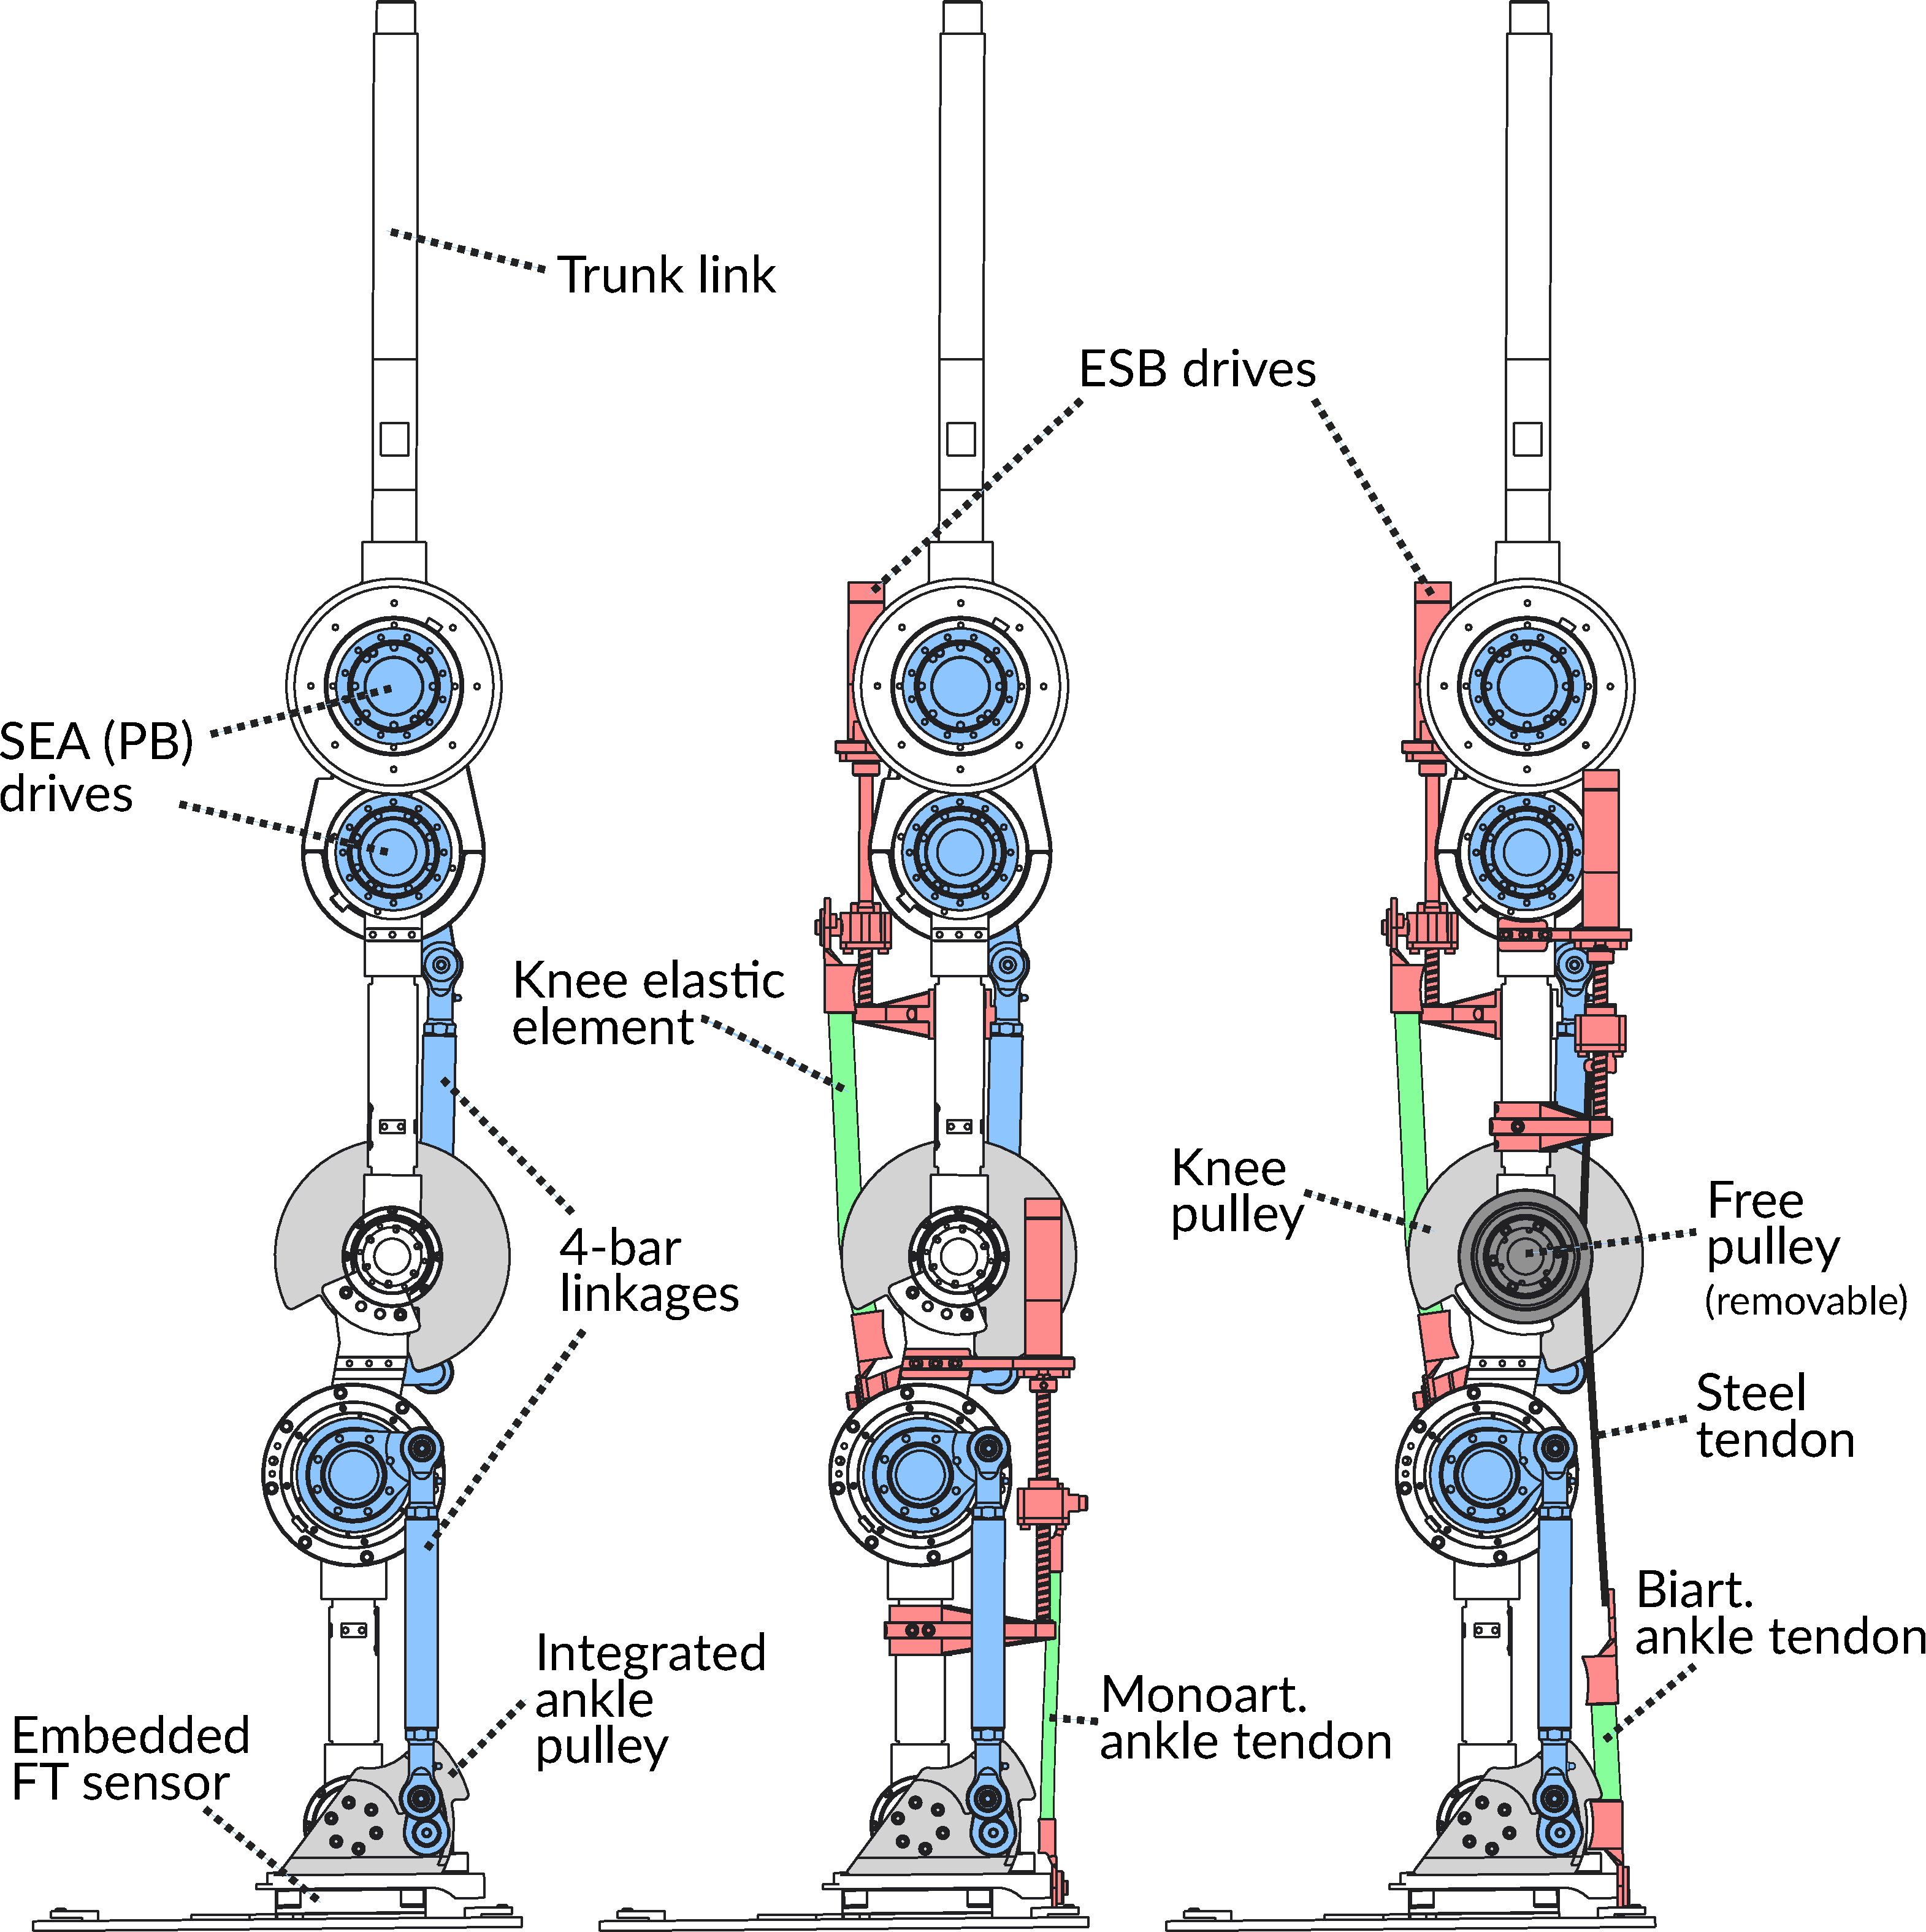
\includegraphics[width=0.98\linewidth]{cad}
	\caption{CAD: SEA-only, mono- and biarticulated configurations}
	\label{fig:configurations}
\end{figure}

\begin{table}
	\begin{tabular}{l|l|l}
		& \textbf{Length [m]} & \textbf{Mass [kg]} \\
		\hline
		Thigh & 0.350 & 2.79, 3.60, 4.24 \\
		Shank & 0.350 & 3.08, 3.91, 3.20 \\
		Foot & 0.063 & 1.70 \\
	\end{tabular}
	\caption{Dimensions and mass distribution of the robot considered in this paper, which are similar to the human limb. Note the foot dimension is height, not length. Mass values given as SEA only, monoarticulated, and biarticulated configurations, respectively.}
	\label{table:designParameters}
\end{table}

%%%%%%%%%%%%%%%%%%%%%%%%%%%%%%%%%%%%%%%%%%%%%%%%%%%%%%%%%
\section{Modelling} 
\label{sec:modelling}

\subsection{Leg Model: Forward Dynamics} 
The leg model, shown in Fig. \ref{fig:Leg_3DoF_model}, consists of four links which are connected by the actuated ankle, knee and hip joints, denoted $q_1,q_2,q_3$, with net actuation torques $\tau_1,\tau_2,\tau_3$. The links have masses $m_1,m_2,m_3,m_4$ and rotational inertiae $J_1,J_2,J_3,J_4$. Their centre of mass (CoM) is assumed to be located on the line connecting the proximal and distal joints at a distance of $r_1,r_2,r_3,r_4$ from the proximal joint for all links except for the foot due to the floating base. %Together, the configurations of the bodies describe the system:
%\begin{equation}
%	\mathbf{x} = [x_1,y_1,\theta_1,x_2,y_2,\theta_2, x_3,y_3,\theta_3,x_4,y_4,%\theta_4]^T. 
%\end{equation}
The Euler-Lagrange formulism with generalised coordinates $\mathbf{q} \in \mathfrak{Q} \subset \mathfrak{R}^{6}$ is used to derive the dynamic equations, with
\begin{equation}
	\mathbf{q} = [x_1,y_1,\theta_1,q_1,q_2,q_3]^T,
	\label{eq:q}
\end{equation}
leading to:
\begin{equation}
	M(\mathbf{q}) \, \mathbf{\ddot q} = \mathbf{\boldsymbol{\tau}} + \mathbf{g}(q) - C(\mathbf{q, \dot q}) \, \mathbf{\dot q} - D \, \mathbf{\dot q} + J_{GRF}^T \, \mathbf{f}_{GRF}.
\label{eq:fwddyn}
\end{equation}

% Figure Leg model
\begin{figure}[ht]
	\centering
	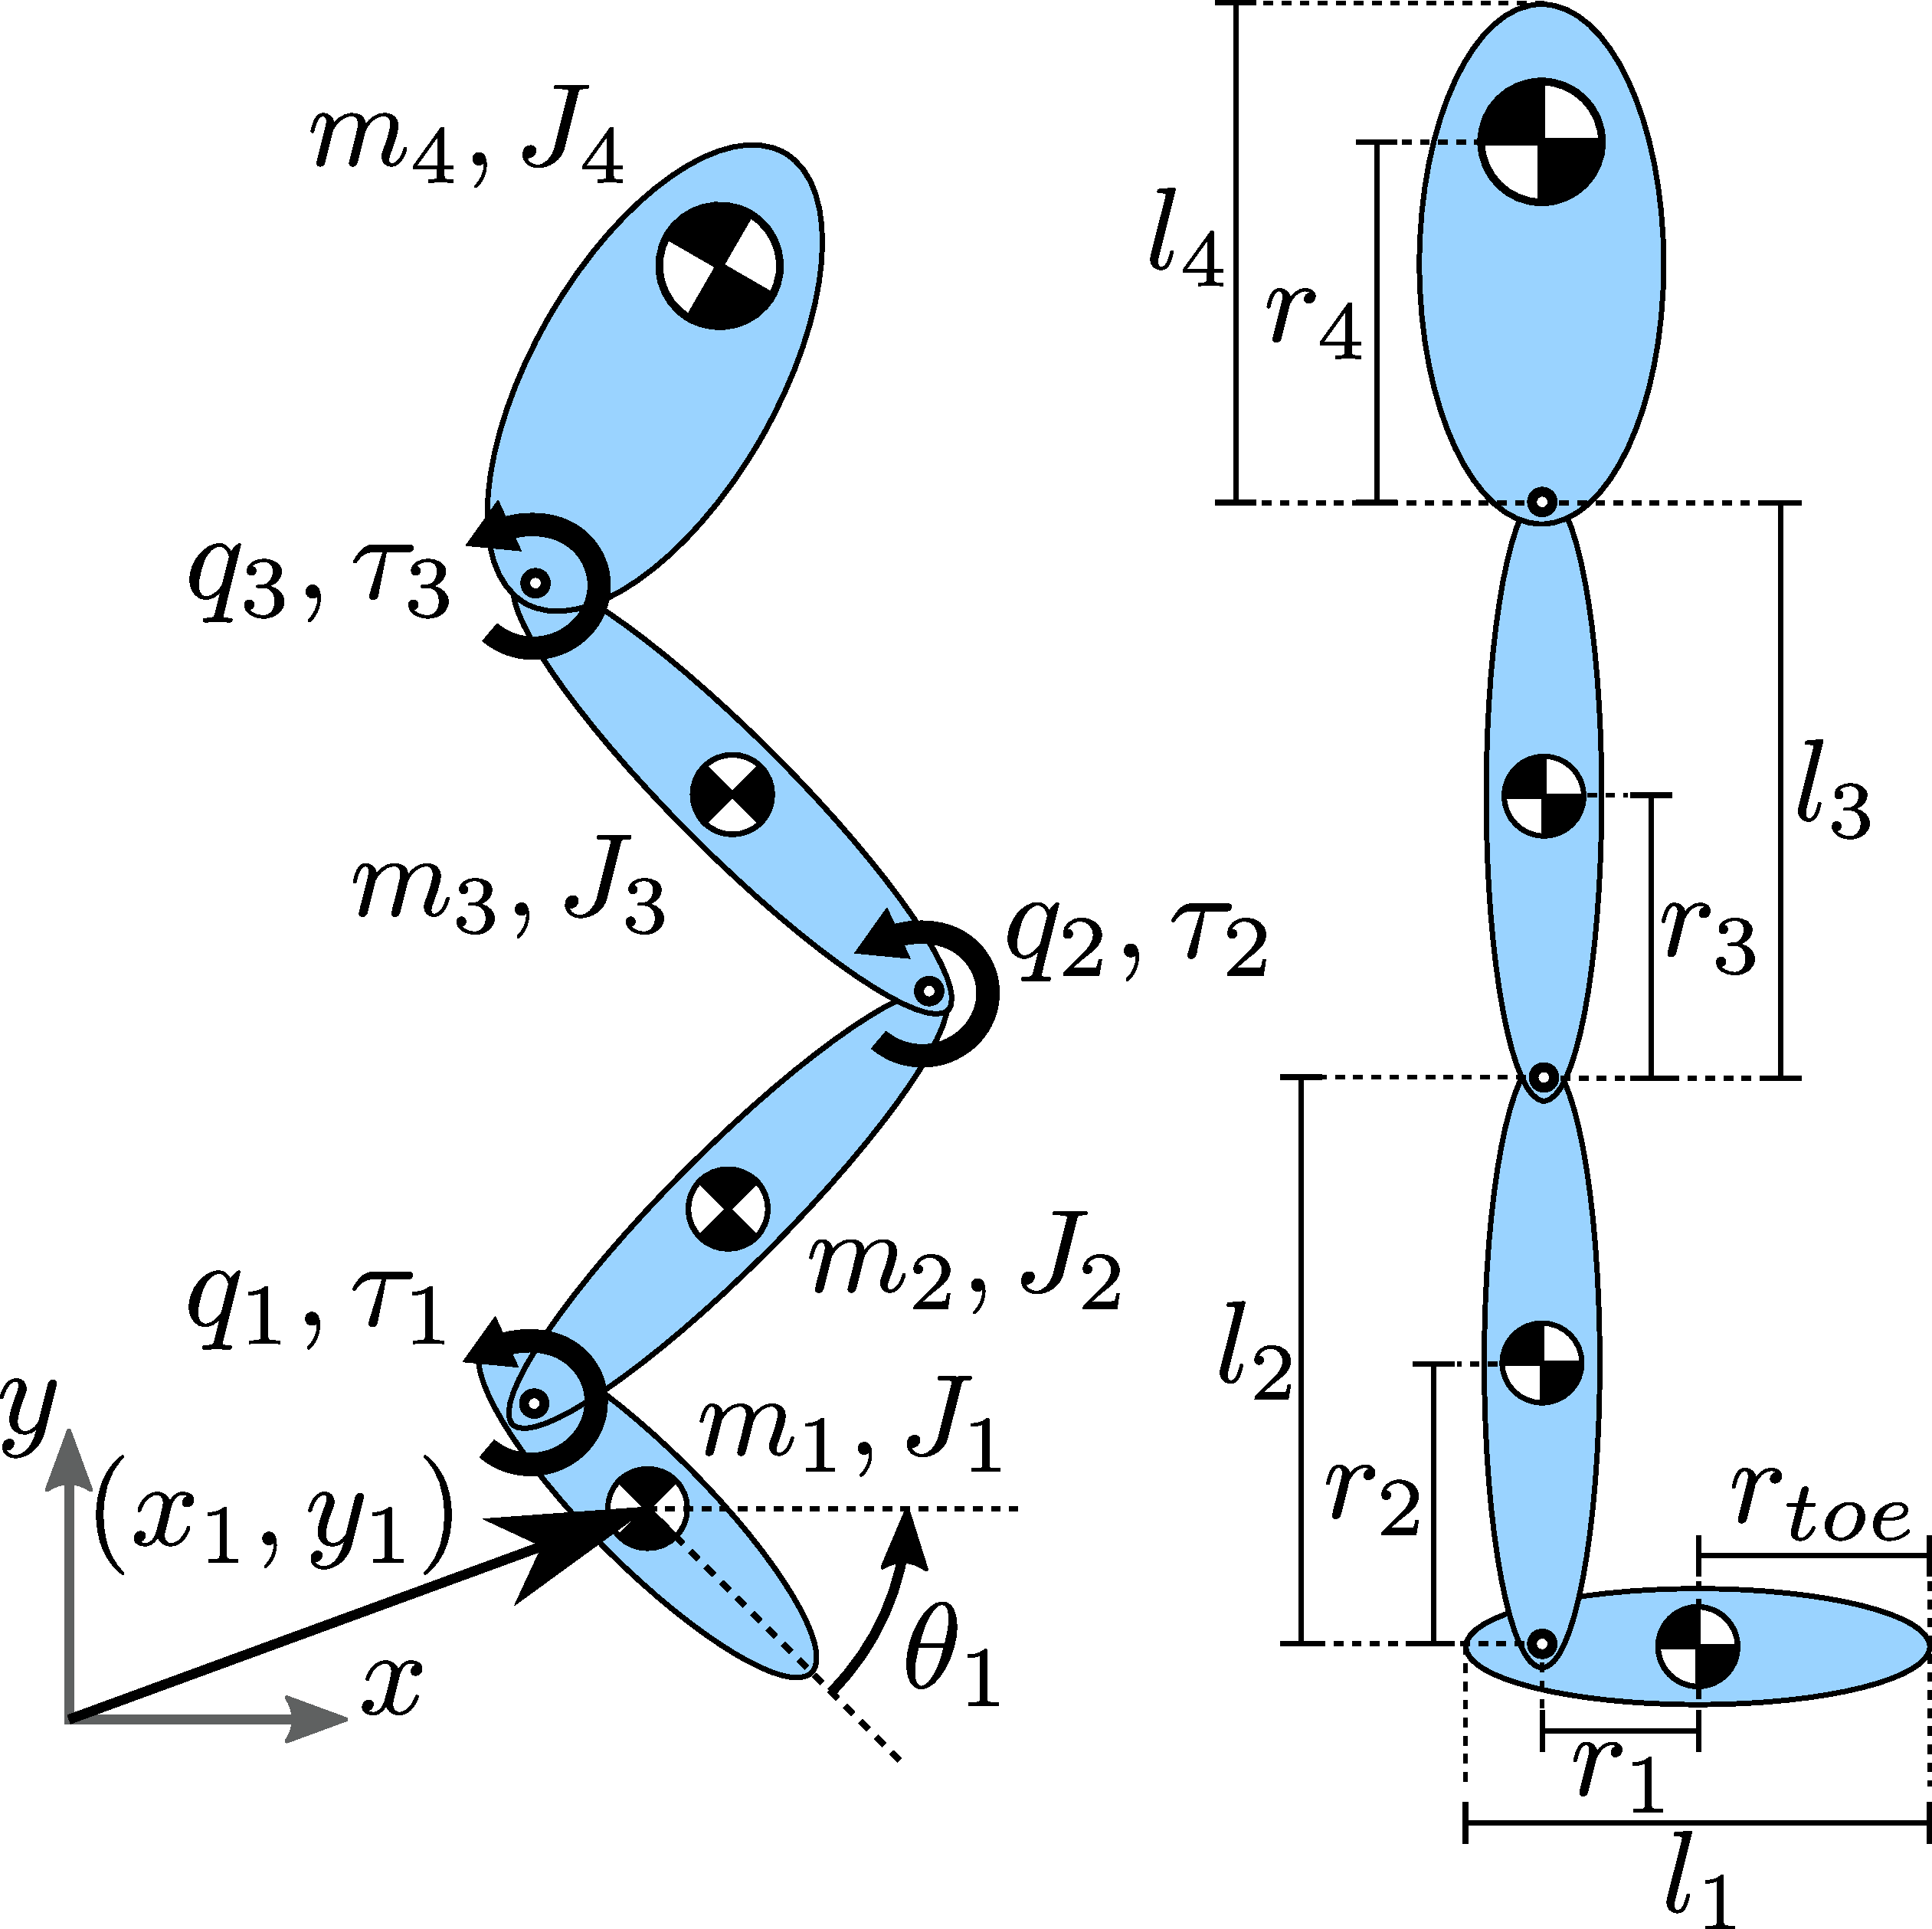
\includegraphics[width=0.6\linewidth]{Leg_3DoF_model}
	\caption{Leg model with floating base. The straight configuration on
		the right corresponds to $\mathbf{q} = \mathbf{0}$.}
	\label{fig:Leg_3DoF_model}
\end{figure}

Here, the damping matrix is denoted by $D = \mathrm{diag} (0,0,0,d_1,d_2,d_3)$, the generalised actuation forces are denoted by $\boldsymbol{\tau} = [0,0,0,\tau_1,\tau_2,\tau_3]^T$, the generalised gravitational forces are denoted by $\mathbf{g(q)}$, and the Coriolis and generalised inertia matrices are denoted by $C\mathbf{(q, \dot q)}$ and $M(\mathbf{q})$, respectively. The Jacobian for the heel and toe is denoted by $J_{GRF}^T$, and the ground reaction forces (GRF) in generalised coordinates are subsequently expressed as $J_{GRF}^T \, \mathbf{f}_{GRF}$. Spring-dampers define $\mathbf{f}_{GRF}$ in the vertical direction and Coulomb and viscous friction define the horizontal component, proportionally to the vertical forces.

\subsection{Leg Model: Inverse Dynamics}
For formulation of the optimisation problem described in Sec. \ref{sec:dynamicOptimisation}, we first derive the inverse dynamics of the system in order to compute the applied active torques \cite{nakanishi2007inverse}. The configuration vector $\mathbf{q}$ can be split in its passive and active joint components, $\mathbf{q}_p$ and $\mathbf{q}_a$, respectively:
\begin{equation}
\mathbf{q} =
\begin{bmatrix}
	\mathbf{q}_p \\
	\mathbf{q}_a
\end{bmatrix},
\end{equation}
with
\begin{equation}
	\mathbf{q}_p = [x_1,y_1,\theta_1]^T, \quad  
	\mathbf{q}_a = [q_1,q_2,q_3]^T.
\end{equation}
\noindent
Similarly, $\boldsymbol{\tau} = \left[\mathbf{0},\boldsymbol{\tau}_a\right]^T$. Substituting these into \eqref{eq:fwddyn} yields:
\begin{equation}
	\begin{aligned}
		&\left[\begin{array}{cc}  
		M_{pp} & M_{pa}\\
		M_{ap} & M_{aa}
		\end{array} \right]
		\left[\begin{array}{c}  
		\mathbf{\ddot q}_p\\
		\mathbf{\ddot q}_a
		\end{array} \right] +
		\left[\begin{array}{c}  
		\mathbf{b}_p \mathbf{(q,\dot q)}\\
		\mathbf{b}_a \mathbf{(q,\dot q)}
		\end{array} \right] 
		=\\
		&\left[\begin{array}{c}  
		\mathbf{0}\\
		\boldsymbol{\tau}_a
		\end{array} \right] 
		+
		J_{GRF}^T \mathbf{f}_{GRF} \, \mathbf{(q, \dot q)},
	\end{aligned}
	\label{eq:ik}
\end{equation}		
where $\mathbf{b}_p$ and $\mathbf{b}_a$ denote the gravitational, Coriolis and damping terms. 
Rearranging \eqref{eq:ik}:
\begin{equation}
	\begin{aligned}
		&\left[\begin{array}{cc}  
		M_{pp} & 0\\
		M_{ap} &-I
		\end{array} \right]
		\left[\begin{array}{c}  
		\mathbf{\ddot q}_p\\
		\boldsymbol{\tau}_a
		\end{array} \right] =\\ 
		-&
		\left[\begin{array}{c}  
		M_{pa}\\
		M_{aa}
		\end{array} \right] 
		\mathbf{\ddot q}_a-
		\mathbf{b(q, \dot q)}+
		J_{GRF}^T \mathbf{f}_{GRF}\mathbf{(q, \dot q)},
	\end{aligned}
\end{equation}	
where $I$ denotes the identity matrix, we obtain the passive joint accelerations $\mathbf{\ddot q}_p$ and active joint torques $\boldsymbol{\tau}_a$ by inversion of the left-hand side mass matrix.


\subsection{Actuation Modelling}
\label{subsec:actuationModel}
As described in Section \ref{sec:legDesign}, three different actuation configurations are considered. In the general monoarticulated ESB case shown in Fig. \ref{fig:ACA}, let $r_p$ denote pulley radius (with sign indicating positive direction) and let $p$ denote the position of motor M2. Given a joint configuration $q$, the elongation of the \textit{ESB} elastic element is given by $\Delta_p = p + r_p q$. Note that the element, with stiffness $k_p$ and damping $d_p$, only applies elastic force under extension as it is of a rubber type material:
\begin{equation}
	F_p =	\left\lbrace
	\begin{array}{ll}
	k_p \, \Delta_p + d_p \, \dot{\Delta}_p	\hspace{0.4cm} & \Delta_p > 0\\
	d_p \, \dot{\Delta}_p & \text{otherwise}
	\end{array}
	\right.
	\label{eq:F_p}
\end{equation}   
As such, the \textit{ESB} generates a torque on the joint equal to $\tau_p = -r_p \, F_p$. From this follows the ankle and knee joint torques for the monoarticulated leg in Fig. \ref{fig:configurations}:
\begin{equation}
	\begin{aligned}
		\tau_1 &= \tau_{SEA,1} - r_{ankle} \, F_{p,1}(p_1,q_1), \\
		\tau_2 &= \tau_{SEA,2} - r_{knee} \, F_{p,2}(p_2,q_2), \\
	\end{aligned}
\end{equation}
where $\tau_{SEA,i}$ denote contributions from the SEAs, $r_\circ$ denote pulley radii, $F_{p,\circ}$ denote linear tendon forces, and $p_i$ denote the respective pretension positions of the \textit{ESB} motors.

For the biarticulated leg configuration shown in Fig. \ref{fig:configurations}, the ankle tendon also spans the knee joint, and the elongation of the \textit{ESB} elastic element is thus given by:
\begin{equation}
	\Delta_{p,1} = p_1 + r_{ankle} \, q_1 + r_{knee,bi} \, q_2,
	\label{eq:Delta_p_biart}
\end{equation}
where $r_{knee,bi}$ denotes the free pulley on the knee. This leads to the ankle and knee torques for the biarticulated case:
\begin{equation}
	\begin{aligned}
		\tau_1 &= \tau_{SEA,1} - r_{ankle} \, F_{p,1}(p_1,q_1,q_2), \\
		\tau_2 &= \tau_{SEA,2} - r_{knee} \, F_{p,2}(p_2,q_2) - r_{knee,bi} \, F_{p,1}(p_1,q_1,q_2).
	\end{aligned}
\end{equation}
Observe that the linear tendon force $F_{p,1}$ is dependent on the configuration of both the knee and ankle joints, and that the tendon applies torque on both joints.
Note that in simulation we model both actuation branches using full motor models with rotor inertiae, friction, current and voltage limitations, high-level joint impedance control, and low-level \textit{SEA} torque control. For details, we refer the reader to \cite{roozing2016design}.


%%%%%%%%%%%%%%%%%%%%%%%%%%%%%%%%%%%%%%%%%%%%%%%%%%%%%%%%%
\section{Dynamic Optimisation} 
\label{sec:dynamicOptimisation}
Finding an optimal motion requires finding the active joint trajectories over time. Expressing these trajectories over time directly poses an extremely high dimensional problem. Hence, we reformulate it from a large scale optimal control problem into a low dimensional parameter optimisation problem \cite{kaphle2008optimality}. We proceed as follows. Sec. \ref{subsec:trajectoryParametrization} describes parametrisation of the joint trajectories, and Sec. \ref{subsec:objectiveCriteria} describes the objective criteria. Lastly, the optimisation algorithm is described in Section \ref{subsec:algorithm}.

\subsection{Trajectory Parametrization} 
\label{subsec:trajectoryParametrization}
A common approach to reduce the dimensionality of trajectory optimisation problems is through basis splines, or $B$-splines, combined with a time-scale factor \cite{ude2000planning,babivc2009biarticulated,wang1999weight,albro2001optimal}. For each joint, the trajectory is described by basis functions $B$ and control points $\mathbf{c}$. For the set of $n$ control points $\mathbf{c}=\left[c_1,\dots,c_n\right]$ evenly spaced over time and basis functions $B_i$, the trajectory for each joint $q_\circ$ assumes the form
\begin{equation}
	q_\circ(t,\mathbf{c}) = \sum_{i=1}^{n} B_i (t) \, c_in
\end{equation}
resulting in $3 \, n$ optimisation variables. The corresponding $B$-splines describe the optimal joint trajectories, velocities, and accelerations over time.

\subsection{Objective Criteria} 
\label{subsec:objectiveCriteria}
The objective function is comprised of three criteria which 1) reward jumping height, 2) penalize used torque, and 3) maintain postural stability of the leg. A minimization of the objective functions with these criteria is represented by:
\begin{equation}
	\min_{\mathbf{c}, \mathbf{p}} J = -J_{performance} + J_{torque} + J_{stability}
\end{equation}
As elaborated in Sec. \ref{subsec:actuationModel}, pretension of the parallel elastic elements can be adjusted, changing the torque--angle relationship and thus allowing use of energy storage to obtain different jumping behaviours. Hence, we add the pretension positions $\mathbf{p}$ as a optimisation variables for the mono- and biarticulated configurations.

In the following, $\gamma_1 \dots \gamma_5$ denote scaling constants.

\subsubsection{Performance}
For jumping performance of the leg we consider the maximum $y$-coordinate of the CoM of the leg with respect to ground, as follows:
\begin{equation}
	J_{performance} = \gamma_1 \: y_{CoM,max}^2
\end{equation}

%For the performance of the leg we distinguish two different objectives: 
%\begin{enumerate}
%	\item Jumping to a certain height efficiently, where the maximum $y$-coordinate reached by the CoM of the leg $y_{COM}$ is to equal a set height $y_{COM}'$ and the energy use is to be minimized:
% \begin{equation}
%	J_{performance} =  c_1 \cdot E^2 + c_2 \cdot |y_{COM}'-y_{COM}|
% \end{equation}
%	Here, $E$ is defined as the cumulative electrical energy consumption in Joules according to the integrated positive power model \cite{verstraten2016energy}:
%	 \begin{equation}
%	E_{elec,pos} = \int max(0,P_{source}(t))dt
%	\end{equation}
%\end{enumerate}

\subsubsection{Torque}
%The active torques pose a problem as the upper and lower bound constraints on the applied torques can become non-linear. Therefore it is chosen to express the torque limits by means of a penalty function in the objective criteria and to only terminate the simulation when the utmost torque limits are violated.
To ensure effective utilisation of elastic energy storage and minimised electrical energy expenditure, the active SEA torque is minimised. We compute the squared $l_2$-norm of the torque contribution of the SEAs, removing the \textit{ESB} contributions from the net active joint torques:
%the realised values of $\boldsymbol{\tau}_a$ computed in Section \ref{sec:modelling} while eliminating the influence of the \textit{ESB}s:  
\begin{equation}
	J_{torque}= \gamma_2 \: \| \boldsymbol{\tau}_a - \boldsymbol{\tau}_{ESB} \|_2^2
\end{equation}
Furthermore, the optimisation algorithm elaborated in Sec. \ref{subsec:algorithm} requires the SEA torques to stay within limits defined by the current limits of the physical system.

\subsubsection{Stability}
To ensure stable jumps, a stability criterion is introduced. This criterion minimises several terms: 1) Mean and final horizontal deviation of the CoM to ensure vertical jumping motion, and 2) Rotational momentum $L$ of the robot at the maximum CoM height.
%\begin{itemize}
%	\item Mean and final horizontal deviation of the CoM to ensure vertical jumping motion;
%	\item Rotational momentum $L$ of the robot at the maximum CoM height.
%\end{itemize}
%The leg posture is considered stable when the $x$-coordinate of the CoM of the leg is equal to its initial $x$-coordinate at the end of the jump, i.e. when the CoM reaches its maximum height. Also, the motion is assumed to be stable when the mean value of the absolute x-coordinates of the CoM equals zero. Higher stability is also assumed for a low rotational momentum $L$ at maximum height of CoM.
These are achieved with the minimization of:
\begin{equation}
	\begin{aligned}
		J_{stability} & =  \gamma_3 \, \left[ x_{CoM}(t_h) - x_{CoM}(t_0) \right]^2 \\
		& + \gamma_4 \, \sum^{N}_{i=1}\frac{| x_{CoM}(t)_i |}{N}^2   
+ \gamma_5 \, L(t_h)^2,
	\end{aligned}
\end{equation}
where $N$ denotes the number of time segments, $t_0$ denotes starting time, and $t_h$ denotes the time where the CoM reaches its maximum height. Let $t_f$ denote the final time, where either the maximum CoM height $y_{CoM,max}$ is reached or the leg has fallen over. For successful jumps $t_h=t_f$.

\subsection{Algorithm}
\label{subsec:algorithm}
Having set up the forward and inverse dynamics and optimisation criteria, we proceed to describe the optimisation algorithm. The algorithm, shown in Algorithm \ref{algo}, takes a simple hand-tuned jumping trajectory as initial guess. Its control points serve as the algorithm input. Initial pretensions are set to $1 \cdot 10^{-4}$ m if present. Each simulation is concluded when the CoM reaches its highest point and the vertical CoM velocity turns negative for successful jumps, or when the leg has fallen over for unsuccessful jumps. 

\begin{algorithm}[ht]
	\caption{Algorithm for joint trajectory optimization} \label{algo}
	\begin{algorithmic}[1]
		\STATE Generate joint reference trajectories with $B$-splines \label{algbegin}
		\IF{joint limits are not exceeded}
			\STATE {Continue} 
		\ELSE
			\STATE Vary optimisation variables, \textbf{go to} \ref{algbegin}
		\ENDIF
		\WHILE{$\dot y_{CoM} > 0$ \AND \textit{not fallen over}}
			\STATE{Run simulation of motion through forward dynamics}
		\ENDWHILE
		\IF{\textit{not fallen over} \AND $\mathrm{max}(|\boldsymbol{\tau}(t)|) < \tau^{max} \quad \forall \: t$}
			\STATE{Continue}
		\ELSE
			\STATE Vary optimisation variables, \textbf{go to} \ref{algbegin}
		\ENDIF
		\STATE Evaluate objective function
		\IF{local minimum reached}
			\STATE{Exit}
		\ELSE
			\STATE Vary optimisation variables, \textbf{go to} \ref{algbegin}
		\ENDIF
	\end{algorithmic}
\end{algorithm}


%%%%%%%%%%%%%%%%%%%%%%%%%%%%%%%%%%%%%%%%%%%%%%%%%%%%%%%%%
\section{Results \& Discussion} \label{sec:results}
The optimisation was performed using a maximum duration of 0.4 seconds, with initial trajectory shown in Fig. \ref{fig:seq}. Computations were performed in MATLAB R2016b, with \texttt{fmincon} as the optimiser function. The weighing constants $\gamma_1 \dots \gamma_5$ were chosen as $\gamma_1=5 \cdot 10^{2} \,, \gamma_2=1.5 \cdot 10^{-4} \,, \gamma_3=1.5 \cdot 10^{3} \,, \gamma_4 = 1\cdot 10^{2}\,$, and $\gamma_5 = 1$.

Results for all three actuation configurations are shown in Fig. \ref{fig:opt_results}, which reports the objective criterion evolution and resulting joint trajectories, torques, power and \textit{ESB} tendon energy storage over time. The results are summarised numerically in Table \ref{table:maxheight}, showing maximum and change in CoM height, pretension positions, cost function $f$ and criteria values, and consumed energy $E_{\text{consumed}}$. The video that accompanies this paper visualises the optimised jumping motions of all three actuation configurations.

% initial guess
\begin{figure}[ht]
	\centering
	%      \framebox{\parbox{3in}
	{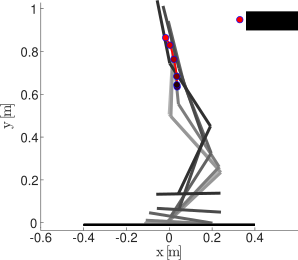
\includegraphics[width=0.55\linewidth]{initialguess_edited}
	}%}	
	\caption{Initial motion used as starting value for the optimisation.}
	\label{fig:seq}	
\end{figure}

\begin{table*}[ht]
	\caption{Jumping optimization results for SEA only, monoarticulated, and biarticulated configurations, respectively.}
	\label{table:maxheight}
	\begin{center}
		\begin{tabular}[t]{c|c|c|c|c|c|c|c|c|c}
			Configuration &  $y_{\text{\textit{CoM}}}^{\text{\textit{max}}}$ [m] & $y_{\text{\textit{CoM}}}^{\text{\textit{initial}}}$ [m]& $y_{\text{\textit{CoM}}}^{\text{\textit{change}}}$ [m]& $p_1,p_2$ [m] & \textit{f} & $E_{\text{\textit{consumed}}}$ [J] & $J_{\text{\textit{performance}}}$ & $J_{\text{\textit{stability}}}$ & $J_{\text{\textit{torque}}}$ \\ 
			\hline
			SEA only	& 0.917 & 0.760 & 0.157 & No \textit{ESB}s	& -370.26 & 805.66 & 426.16 & 0.85 & 55.05\\
			\hline
			Mono.		& 0.951 (+4\%) & 0.703 & 0.247 & 0.060, -0.014	& -402.90 & 567.64 & 451.77 & 1.26 & 47.61 \\
			\hline
			Bi.			& 1.013 (+10\%) & 0.724 & 0.290 & 0.044, 0.029		& -478.73 & 867.35 & 526.27 & 0.96 & 46.58
		\end{tabular}
	\end{center}
\end{table*}


% Large figure with all the optimisation results
\begin{figure*}[ht]
	\centering
	
	% Criteria evolution
	\begin{subfigure}[t]{0.32\linewidth}
		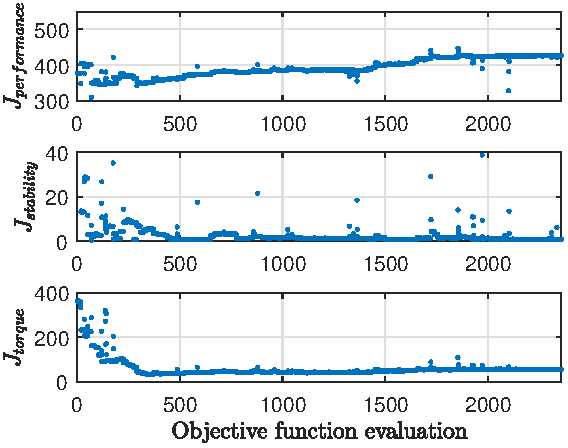
\includegraphics[width=\linewidth]{noESB/crit_high}
		\caption{No ESB: Criterion evolution.}
		\label{fig:noESB_crit_high}
	\end{subfigure}
	%
	\begin{subfigure}[t]{0.32\linewidth}
		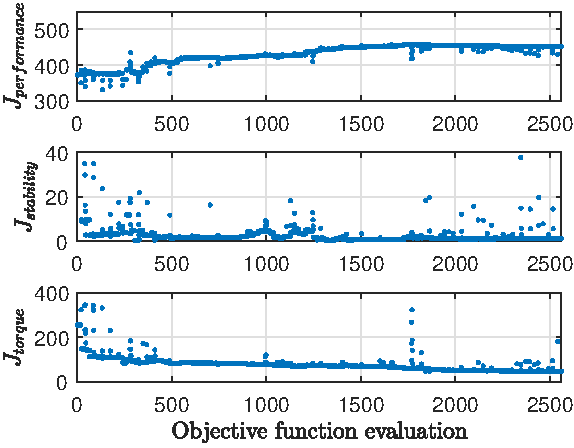
\includegraphics[width=\linewidth]{mono/crit_high}
		\caption{Monoarticulated: Criterion evolution.}
		\label{fig:mono_crit_high}
	\end{subfigure}
	%
	\begin{subfigure}[t]{0.32\linewidth}
		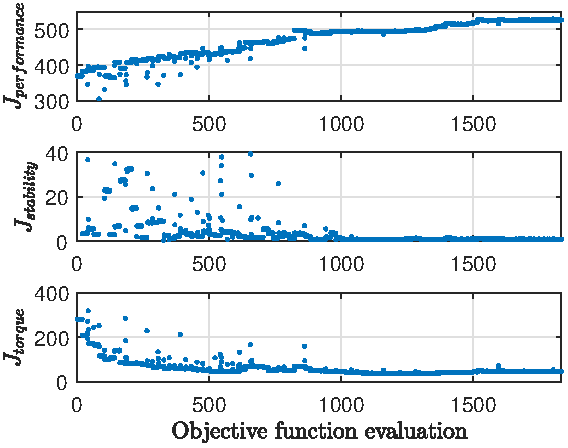
\includegraphics[width=\linewidth]{bi/crit_high}
		\caption{Biarticulated: Criterion evolution.}
		\label{fig:bi_crit_high}
	\end{subfigure}
	
	\vspace{1mm}
	
	% Trajectories
	\begin{subfigure}[t]{0.32\linewidth}
		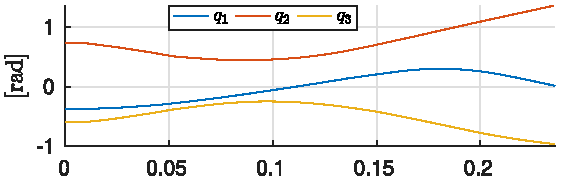
\includegraphics[width=\linewidth]{noESB/final_traj}
		\caption{No ESB: Joint trajectories.}
		\label{fig:noESB_traj}
	\end{subfigure}
	%
	\begin{subfigure}[t]{0.32\linewidth}
		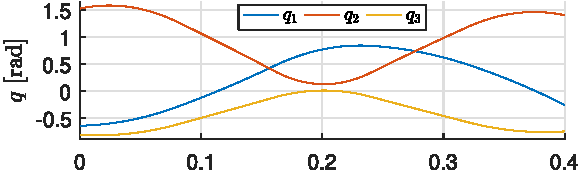
\includegraphics[width=\linewidth]{mono/final_traj}
		\caption{Monoarticulated: Joint trajectories.}
		\label{fig:mono_traj}
	\end{subfigure}
	%
	\begin{subfigure}[t]{0.32\linewidth}
		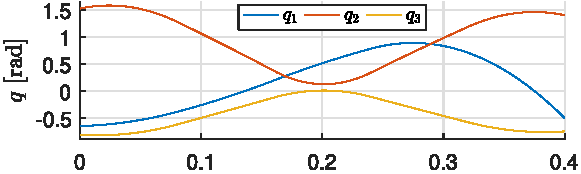
\includegraphics[width=\linewidth]{bi/final_traj}
		\caption{Biarticulated: Joint trajectories.}
		\label{fig:bi_traj}
	\end{subfigure}
	
	\vspace{1mm}
	
	% Ankle torques
	\begin{subfigure}[t]{0.32\linewidth}
		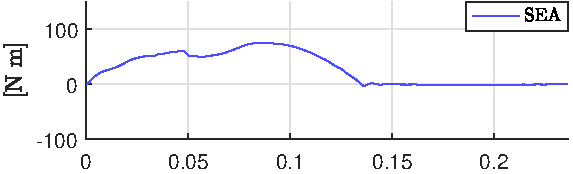
\includegraphics[width=\linewidth]{noESB/q_1_torques}
		\caption{No ESB: Ankle ($q_1$) torques.}
		\label{fig:noESB_q_1_torques}
	\end{subfigure}
	%
	\begin{subfigure}[t]{0.32\linewidth}
		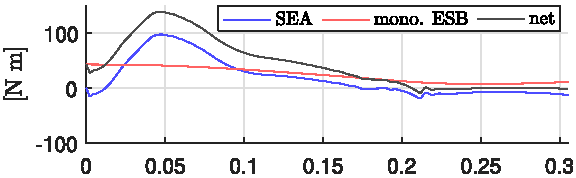
\includegraphics[width=\linewidth]{mono/q_1_torques}
		\caption{Monoarticulated: Ankle ($q_1$) torques.}
		\label{fig:mono_q_1_torques}
	\end{subfigure}
	%
	\begin{subfigure}[t]{0.32\linewidth}
		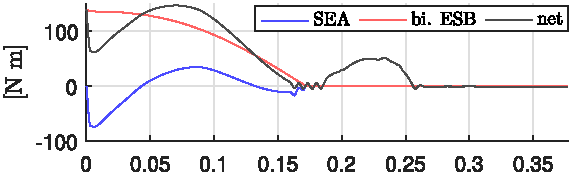
\includegraphics[width=\linewidth]{bi/q_1_torques}
		\caption{Biarticulated: Ankle ($q_1$) torques.}
		\label{fig:bi_q_1_torques}
	\end{subfigure}
	
	\vspace{1mm}
	
	% Knee torques
	\begin{subfigure}[t]{0.32\linewidth}
		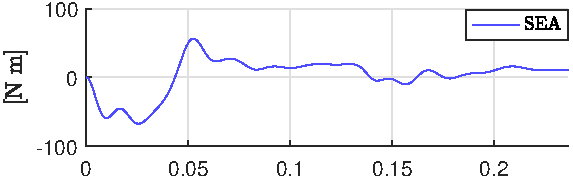
\includegraphics[width=\linewidth]{noESB/q_2_torques}
		\caption{No ESB: Knee ($q_2$) torques.}
		\label{fig:noESB_q_2_torques}
	\end{subfigure}
	%
	\begin{subfigure}[t]{0.32\linewidth}
		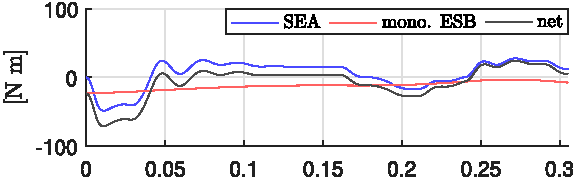
\includegraphics[width=\linewidth]{mono/q_2_torques}
		\caption{Monoarticulated: Knee ($q_2$) torques.}
		\label{fig:mono_q_2_torques}
	\end{subfigure}
	%
	\begin{subfigure}[t]{0.32\linewidth}
		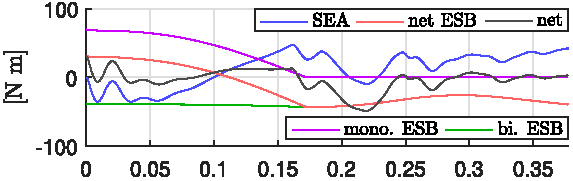
\includegraphics[width=\linewidth]{bi/q_2_torques}
		\caption{Biarticulated: Knee ($q_2$) torques.}
		\label{fig:bi_q_2_torques}
	\end{subfigure}
	
	\vspace{1mm}
	
	% Hip torques
	\begin{subfigure}[t]{0.32\linewidth}
		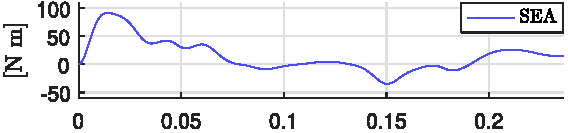
\includegraphics[width=\linewidth]{noESB/q_3_torques}
		\caption{No ESB: Hip ($q_3$) torques.}
		\label{fig:noESB_q_3_torques}
	\end{subfigure}
	%
	\begin{subfigure}[t]{0.32\linewidth}
		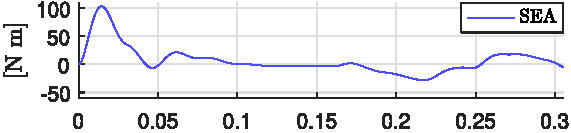
\includegraphics[width=\linewidth]{mono/q_3_torques}
		\caption{Monoarticulated: Hip ($q_3$) torques.}
		\label{fig:mono_q_3_torques}
	\end{subfigure}
	%
	\begin{subfigure}[t]{0.32\linewidth}
		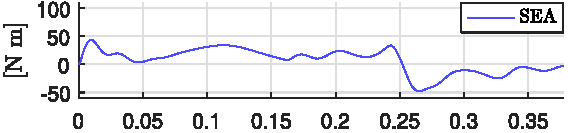
\includegraphics[width=\linewidth]{bi/q_3_torques}
		\caption{Biarticulated: Hip ($q_3$) torques.}
		\label{fig:bi_q_3_torques}
	\end{subfigure}
	
	\vspace{1mm}
	
	% Net Joint power
	\begin{subfigure}[t]{0.32\linewidth}
		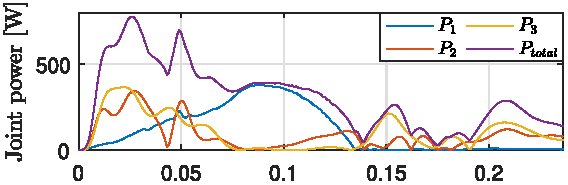
\includegraphics[width=\linewidth]{noESB/P_q}
		\caption{No ESB: Net joint power.}
		\label{fig:noESB_P_q}
	\end{subfigure}
	%
	\begin{subfigure}[t]{0.32\linewidth}
		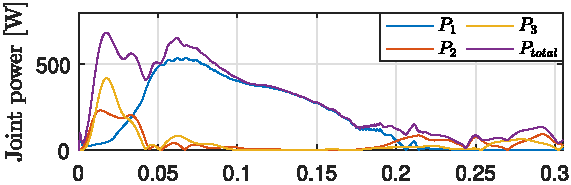
\includegraphics[width=\linewidth]{mono/P_q}
		\caption{Monoarticulated: Net joint power.}
		\label{fig:mono_P_q}
	\end{subfigure}
	%
	\begin{subfigure}[t]{0.32\linewidth}
		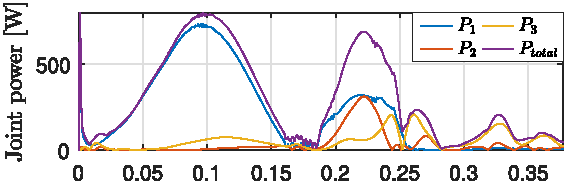
\includegraphics[width=\linewidth]{bi/P_q}
		\caption{Biarticulated: Net joint power.}
		\label{fig:bi_P_q}
	\end{subfigure}
	
	\vspace{1mm}
	
	% ESB storage
	\begin{subfigure}[t]{0.32\linewidth}
		\centering
		\raisebox{0pt}[0pt][0pt]{%
			\raisebox{9mm}{\texttt{~~No ESB tendons.}}%
		}
	\end{subfigure}
	%
	\begin{subfigure}[t]{0.32\linewidth}
		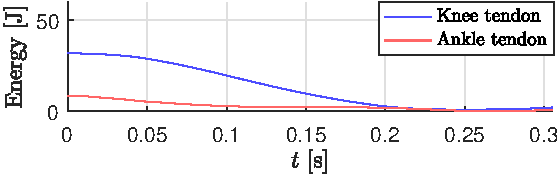
\includegraphics[width=\linewidth]{mono/ESB_storage}
		\caption{Monoarticulated: Tendon energy storage.}
		\label{fig:mono_ESB}
	\end{subfigure}
	%
	\begin{subfigure}[t]{0.32\linewidth}
		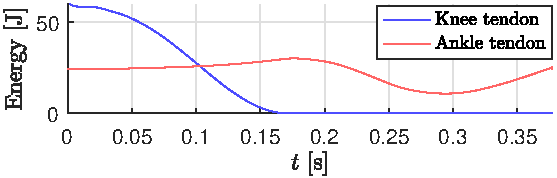
\includegraphics[width=\linewidth]{bi/ESB_storage}
		\caption{Biarticulated: Tendon energy storage.}
		\label{fig:bi_ESB}
	\end{subfigure}
	
	\caption{Final simulation results with optimised motions. Left column: without ESB (SEA only), middle column: monoarticulated configuration, right column: biarticulated configuration. The horizontal axes show the elapsed time in seconds.}
	\label{fig:opt_results}
\end{figure*}

One immediate observation from the results is that ankle extension is one of the primary contributors to vertical momentum, across all three configurations. This is evidenced by the significantly larger joint power compared to the knee (Fig. \ref{fig:noESB_P_q}--\ref{fig:bi_P_q}). We suspect the reason for this is the relatively large amount of ankle torque available (as identical SEAs are used for ankle and knee), combined with the 0.4\,s maximum duration which may not allow for a fully flexed knee at $t=0$. Although the movements for all three configurations are similar, some key differences can be observed:

\begin{enumerate}
	\item \textbf{Joint trajectories}: While the mono- and biarticulated configurations use knee extension at approximately 0.2 seconds into the motion to obtain additional vertical momentum of the CoM, knee extension is nearly absent for the configuration without \textit{ESB}. This is likely due to the torque costs for doing so. Furthermore, the no-\textit{ESB} and monoarticulated configurations use hip extension extensively during the early stages of the jump, whereas the biarticulated extends its hip at the end of the upwards motion to increase its CoM height.

	\item \textbf{Ankle torque}: Fig. \ref{fig:noESB_q_1_torques}--\ref{fig:bi_q_1_torques} show that the \textit{PB} ankle torque used by the biarticulated configuration is significantly lower than that of the other configurations, but due to the biarticulated tendon it achieves the highest net ankle torque during extension.
	
	\item \textbf{Joint power}: Fig. \ref{fig:noESB_P_q}--\ref{fig:bi_P_q} show that the biarticulated configuration net joint power exceeds that of the other configurations, particularly for the ankle joint. A comparison with Fig. \ref{fig:mono_ESB} and \ref{fig:bi_ESB} shows that the largest change in power is largely synchronous with release of energy in the \textit{ESB} tendons, demonstrating effective use of the energy storage capacity.
	
	\item \textbf{Power transfer in biarticulation}: The biarticulated tendon is providing positive torque on the knee (i.e. flexing the knee) for the first 0.17\,s (Fig. \ref{fig:bi_q_2_torques}), while the knee is extending. As the stored energy in the biarticulated tendon stays roughly constant, this positive power is not stored but transferred to the ankle, aiding in ankle extension. This demonstrates the effectiveness of the biarticulated tendon.
	
	\item \textbf{Energy consumption}: While the monoarticulated case is able to reach a significant increase of 4\% in jumping height compared to the no \textit{ESB} case, it does so much more efficiently, reducing energy consumption by 30\%. However, in the biarticulated case, while $J_{\text{torque}}$ is further reduced, the consumed energy is increased. This suggests a more elaborate effort penalisation criterion which takes the electrical dynamics of the actuators into account can improve the results further.
\end{enumerate}


%%%%%%%%%%%%%%%%%%%%%%%%%%%%%%%%%%%%%%%%%%%%%%%%%%%%%%%%%
\section{Conclusions} \label{sec:conclusions} 
This paper has presented the optimisation of explosive jumping motions of a 3-DoF leg prototype using both series and parallel compliant articulated actuation. Monoarticulated and biarticulated configurations which are augmented with articulated and adjustable parallel compliance were compared to a state-of-the-art Series-Elastic based actuation structure. The optimisation results show jumps 4\% higher in monoarticulated configuration and over 10\% higher in biarticulated configuration, and reduced torque requirements of the main actuators. Furthermore, the biarticulated case demonstrates the potential of multiarticulated compliance, in terms of higher peak joint power and joint-to-joint power transfer.

While these results are promising, experiments with the recently developed hardware prototype are still underway. Furthermore, in this work only fixed pretension positions of the parallel branches were used. Time-varying pretension positions may improve performance further. These developments and their results will be considered in future works.


%%%%%%%%%%%%%%%%%%%%%%%%%%%%%%%%%%%%%%%%%%%%%%%%%%%%%%%%%
\addtolength{\textheight}{-0cm}   % This command serves to balance the column lengths
                                  % on the last page of the document manually. It shortens
                                  % the textheight of the last page by a suitable amount.
                                  % This command does not take effect until the next page
                                  % so it should come on the page before the last. Make
                                  % sure that you do not shorten the textheight too much.


%%%%%%%%%%%%%%%%%%%%%%%%%%%%%%%%%%%%%%%%%%%%%%%%%%%%%%%%%
\section{ACKNOWLEDGMENT}
Supported by European Commission projects WALK-MAN (611832), CENTAURO (644839), CogIMon (644727)


%%%%%%%%%%%%%%%%%%%%%%%%%%%%%%%%%%%%%%%%%%%%%%%%%%%%%%%%%
% References
\bibliographystyle{ieeetran} % Requires ieeetran.bst
\bibliography{lit}

\end{document}
